
\documentclass[10pt]{article}
\usepackage[%
left=0.984252in,%
right=0.787402in,%
top=0.787402in,%
bottom=0.787402in,%
paperheight=11in,%
paperwidth=8.5in%
]{geometry}%

\usepackage{xeCJK}
\usepackage{blindtext}
\usepackage[T1]{fontenc}
\usepackage{caption}
\usepackage{graphicx}
\usepackage{textcomp}
\usepackage{fancyhdr}
\pagestyle{fancy}
\fancyhf{}
\fancyhead[R]{\thepage}
\usepackage{float}
\usepackage{alltt}

\setCJKmainfont{AozoraMinchoRegular.ttf}
\setCJKsansfont{AozoraMincho-bold.ttf}

\title{オシロスコープ}
\author{18NC021 \thanks{情報通信基礎実験1}}
\date{カトリ スザン}
\captionsetup[table]{name=表}
\captionsetup[figure]{name=図}

\begin{document}

\begin{titlepage}
	\maketitle
\end{titlepage}

\tableofcontents
\pagebreak

\section{目的}
 $\bullet$ オシロスコープは、工学科における一般的な波形観測装置として利用される機会が多いので、その利用法を習得する。

\section{使用機器}

\begingroup
\setlength{\tabcolsep}{5pt} % Default value: 6pt
\renewcommand{\arraystretch}{1.5} % Default value: 1
% Parts list table
\begin{table}[H]
    \centering
	\caption{使用機器}
	\begin{tabular}{|l|l|l|}
	    \hline
	    使用機器 & 会社名 & 型番等\\[0.5ex]
		\hline\hline
		オシロスコープ &IWATU &	SS-7802A \\ \hline
		プローブ	&  &10:1, 1:1 \\ \hline
		波形発生器  &	 &NO.05 \\ \hline
        電気電子計 & NATIONAL &	VP-9631A \\ \hline
	\end{tabular}
\end{table} 
\endgroup

\section{実験 1 波形の測定}

\subsection{実験方法}
$\bullet$ 正弦波、方形波、三角波の 3 種類について測定する。波形発生装置の直流重畳スイッチを off。オシロスコープの DC/AC 切り替えは DC として実験を行うこと

\subsection{回路図}
\begin{figure}[H]
	\centering
	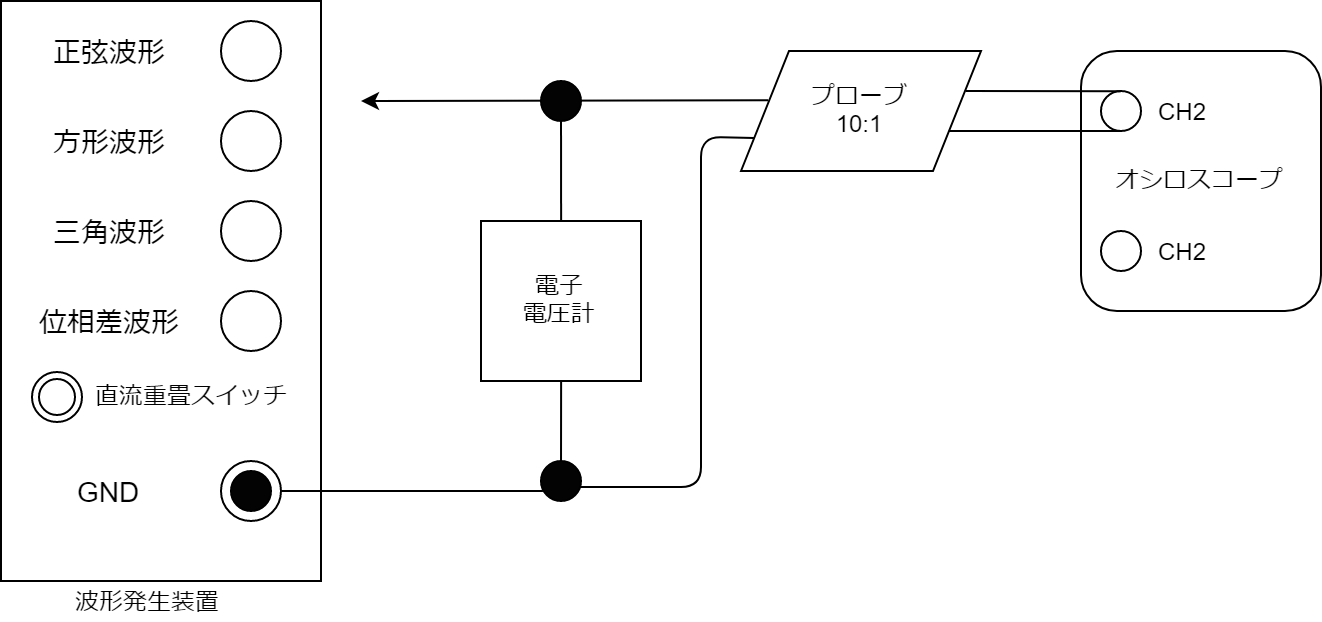
\includegraphics[width=0.704\textwidth]{exp1.png}
	\caption{回路図}
\end{figure}

\subsection{結果}
$\bullet$ 次のページ
\pagebreak

\section{実験 3 波形差の測定}
\subsection{実験方法}
$\bullet$正弦波をCH1に、位相差波形をCH2に接続する。次いでオシロスコープの入力結合切替は「AC」入力選択は「CH1、CH2をONにする」、トリガソースは「CH1」、トリガーリモートは「AUTO」とする。 以上で、2つの波形がCRT上に現れる。CH1の入力切替をGNDにしてグラインドラインを中心より1DIV~2DIV下に設定する、二つの波形の位相関係を見ることができる。2 つの波形より位相差 \(\Phi\) は \\

\begin{center}
    \(\Phi\) = 360B/A (度) で表せる。
\end{center}

\subsection{回路図}
\begin{figure}[H]
	\centering
	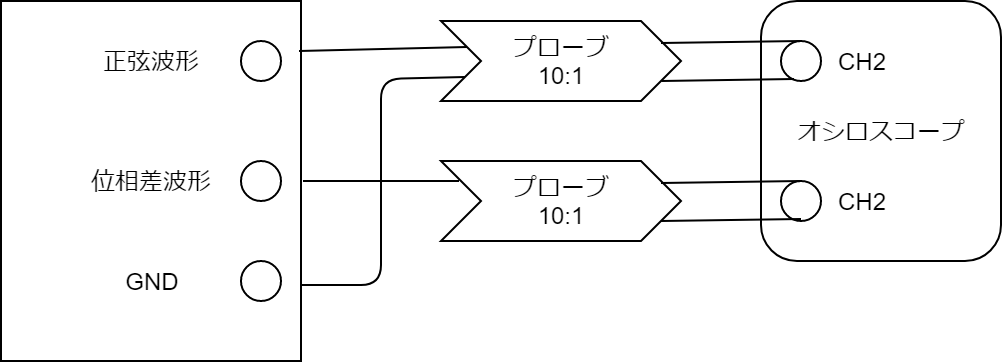
\includegraphics[width=0.704\textwidth]{exp3.png}
	\caption{回路図}
\end{figure}

\subsection{結果}
$\bullet$ 次のページ

\pagebreak

\section{検討事項}

\subsection{検証1}
$\bullet$ 実験1においてスケッチ波形より計算された各種値と、電子電圧計の指示の変換値を次のような一覧表にせよ (波 形による波形率は参考書を参照のこと)。
\begingroup
\setlength{\tabcolsep}{5pt} % Default value: 6pt
\renewcommand{\arraystretch}{1.5} % Default value: 1
% Parts list table
\begin{table}[H]
    \centering
	\caption{実験1の検証}
	
	\hspace{-1.75cm}スケッチ波形より | \hspace{0.2cm}電子電圧計の指示より\\
	\begin{tabular}{|1|l|l|l|l|l|l|l|l|l|}
	    \hline
	    &最大値 & 実効値 & 平均値 & 指示 & 平均値 & 波形率 & 実効値 & 波高率 & 最大値 \\[0.5ex]
		\hline\hline
		正弦波 &10V &7.09V &6.36V &7.09V &6.3V &1.11 &2.21V &1.41 &10V \\ \hline
		方形波	&5.1V &5.1V &5.1V &5.99V &5.1V &1 &1.0V &1.00 &8.4V \\ \hline
		三角波 &5.4V &3.12V &2.7V &3.1V &2.7V &1.15 &3.12V &1.73 &4.37V \\ \hline
	\end{tabular}
\end{table} 
\endgroup

\subsection{検証2}
$\bullet$ 最大値電圧 100V の正弦波の半波整流波形をこの電子電圧計にて測定すると何 V を指示するか。また、全波整流波形の場合は何ボルトを指示するか。
\\
\\
$\bullet$ 正弦波の半波整流形 : 35.3V (Va = 100/\(\Pi\)) \\
$\bullet$ 全波整流波形 : 70.7V (Va = 2 \(\times\) 100 / \(\Pi\))

\section{吟味 (考察)}
$\bullet$ 本実験では今まで電気回路基礎などの授業で学んできた正弦波、三角波や方形波を実際にオシロスコープを使って観測することで、波形の性質の理解がより深まりました。また、二つの位相の違う波をオシロスコープで観測することで、位相角、位相の遅れ、進みがそれぞれ何を意味するかを理解しました。そしてオシロスコープを使って波形の位相や周波数を測定できるようになりました。

\end{document}